\documentclass[../../main.tex]{subfiles}

\graphicspath{{../../image/}{../../figure/}}

\begin{document}

\section{机器学习简史}\label{section:ch01-机器学习简史}

机器学习拥有悠久且丰富的发展历史，涌现了多种不同的研究路径。本节将着重介绍基于神经网络的机器学习方法的发展脉络，因为神经网络构成了深度学习的基石，并且在实际应用中已被证明是最为有效的机器学习方法。

神经网络模型最初受到人类和其他哺乳动物大脑信息处理机制的启发。大脑中处理信息的基本单元是称为神经元的电活性细胞，如\cref{figure:ch01-神经元示意图}所示。当神经元放电时，它会沿着轴突发送电脉冲，到达称为突触的连接点，这些连接点与其他神经元形成连接。在突触处会释放称为神经递质的化学信号，这些信号可以刺激或抑制后续神经元放电。

\begin{definition}[神经元与突触]\label{definition:ch01-神经元与突触}
大脑中处理信息的基本单元是称为\textbf{神经元}（neuron）的电活性细胞。神经元放电时会沿\textbf{轴突}（axon）发送电脉冲，到达称为\textbf{突触}（synapse）的连接点，这些连接点与其他神经元形成连接；在突触处释放的、可以刺激或抑制后续神经元放电的化学信号称为\textbf{神经递质}。
\end{definition}

% SUPPLEMENT: parent=definition:ch01-神经元与突触; kind=motivation; location=紧随其后的 remark（重构新增）
\begin{remark}（重构新增）
这里的描述是生物机制的极度简化：真实的神经元有复杂的树突整合、多种离子通道与时间动态，而本书只保留“加权输入—阈值放电—突触强度可变”这三件事。这样做的动机是：只有把生物细节剥离，才能得到一个可以用少数几个实数（权重）描述、并且可能通过数据调整的数学模型。
需要注意“兴奋／抑制”的作用方向：突触强度可以为正（兴奋）也可以为负（抑制），因此后文的权重 $w_i$ 允许取负值，这是模型能够表示“此消彼长”关系的前提。至于“突触强度的变化是学习与记忆的机制”这一生物学论断，本书只用它作为引入可调参数的动机，并不把它当作需要证明的命题。
\end{remark}

\begin{figure}[htbp]
  \centering
  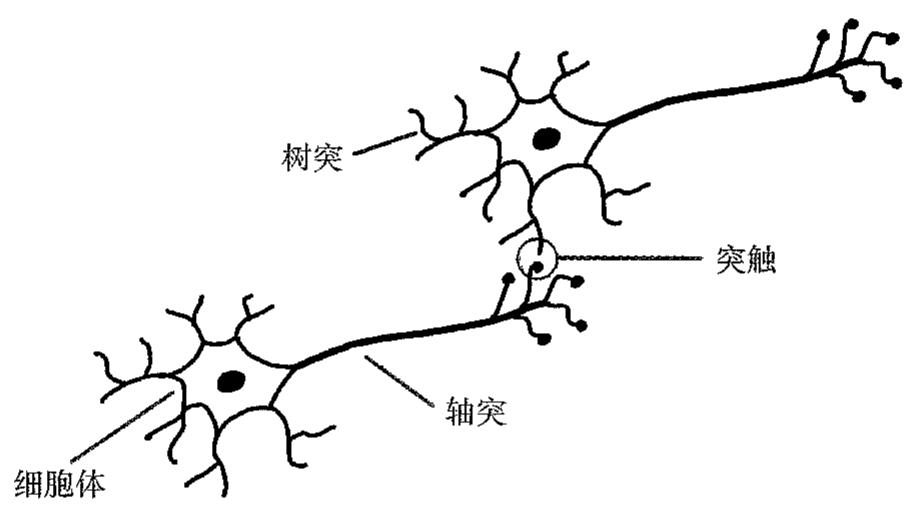
\includegraphics[width=0.6\textwidth]{ch01-fig1-13-neurons.png}
  \caption{人脑中两个神经元的示意图（这些电活性细胞通过称为突触的连接点进行通信，这些连接点随着神经网络的学习而变化）}
  \label{figure:ch01-神经元示意图}
\end{figure}

人脑总共包含约 900 亿个神经元，每个神经元平均与其他数千个神经元通过突触相连，形成了一个包含约 100 万亿（$10^{14}$）个突触连接的复杂网络。如果某个神经元接收到来自其他神经元放电的足够强度的刺激，那么它自身也可能被触发放电。然而，某些突触具有负向调节或抑制作用，即输入神经元的放电会降低输出神经元放电的可能性。一个神经元能否引发另一个神经元的放电取决于突触的连接强度，而这些突触的连接强度的动态变化正是大脑存储信息和进行经验学习的关键机制。

神经元的这些属性已被抽象为简单的数学模型，即人工神经网络（Artificial Neural Network, ANN），它们成为计算学习方法的基础（McCulloch and Pitts, 1943）。诸多此类模型通过对其他神经元的输出的线性组合来描述单个神经元的特性，然后使用非线性函数进行转换。该过程可以用数学表达式表示为：

\begin{definition}[人工神经网络]\label{definition:ch01-人工神经网络}
把神经元的上述属性抽象成的数学模型称为\textbf{人工神经网络}（Artificial Neural Network, ANN）。其中每个单元接收 $M$ 个输入 $x_1,\cdots,x_M$，带有一组权重 $w_1,\cdots,w_M$ 与一个非线性函数 $f(\cdot)$，并按
\begin{align}
  a &= \sum_{i=1}^{M} w_i x_i \label{align:ch01-神经元预激活}\\
  y &= f(a) \label{align:ch01-神经元激活}
\end{align}
计算其输出。其中 $x_1,\cdots,x_M$ 表示与向该神经元发送连接的其他神经元的活动相对应的 $M$ 个输入，$w_1,\cdots,w_M$ 是\textbf{权重}（weight），表示相关突触的强度；量 $a$ 称为\textbf{预激活}（pre-activation），非线性函数 $f(\cdot)$ 称为\textbf{激活函数}（activation function），输出 $y$ 称为\textbf{激活}（activation）。
\end{definition}

% SUPPLEMENT: parent=definition:ch01-人工神经网络; kind=motivation; location=紧随其后的 remark（重构新增）
\begin{remark}（重构新增）
这个模型抓住了生物神经元的两件事：先对所有输入作加权求和（线性组合），再作一次非线性变换。前者对应“突触强度决定影响力”，后者对应“达不到阈值就不放电”。缺了非线性，多层叠加仍等价于单层线性模型（\cref{definition:ch01-线性模型}），网络就失去了表达能力；因此 $f$ 的非线性是整个结构的要害。
条件上要注意式\eqref{align:ch01-神经元预激活}中没有偏置项：只有在补充一个恒为 $1$ 的输入并把对应权重当作阈值时，才能表示“总加权输入超过某个非零阈值才放电”的情形。此外权重 $w_i$ 可正可负，这正是前面所说兴奋性与抑制性突触的数学对应。
\end{remark}

可以看出，式\eqref{align:ch01-多项式模型}可视为这个模型的一个特例，其中输入 $x_i$ 由单一变量 $x$ 的各次幂构成，而激活函数 $f(\cdot)$ 退化为恒等函数 $f(a)=a$。

\begin{proposition}[多项式函数是神经元模型的特例]\label{proposition:ch01-多项式是神经元特例}
在\cref{definition:ch01-人工神经网络}中取
\begin{align*}
  x_i = x^{i}\quad (i=1,\cdots,M),\qquad f(a)=a,
\end{align*}
则该单元的输出为 $y=\sum_{i=1}^{M} w_i x^{i}$，即式\eqref{align:ch01-多项式模型}中常数项取 $w_0=0$ 时的多项式函数。若再补充一个恒等于 $1$ 的输入 $x_0\triangleq 1$ 并把 $w_0$ 取为该输入的权重，则式\eqref{align:ch01-多项式模型}的完整形式也是这个模型的特例。
\end{proposition}

\begin{proof}（重构新增）
把 $x_i=x^{i}$ 与 $f(a)=a$ 代入式\eqref{align:ch01-神经元预激活}与式\eqref{align:ch01-神经元激活}，得
\begin{align*}
  a = \sum_{i=1}^{M} w_i x^{i},
  \qquad
  y = f(a) = a = \sum_{i=1}^{M} w_i x^{i},
\end{align*}
这正是式\eqref{align:ch01-多项式模型}中求和从 $j=1$ 开始的特殊情形，也就是 $w_0=0$ 的情形。
若把输入编号推广为 $i=0,1,\cdots,M$ 并令 $x_0=1$，则和式变为 $\sum_{i=0}^{M} w_i x^{i}=w_0+\sum_{i=1}^{M} w_i x^{i}$，与式\eqref{align:ch01-多项式模型}完全一致，故完整的多项式函数同样是该模型的特例。
\end{proof}

% SUPPLEMENT: parent=proposition:ch01-多项式是神经元特例; kind=motivation; location=紧随其后的 remark（重构新增）
\begin{remark}（重构新增）
这条命题说明：多项式拟合并不是与神经网络并列的另一类方法，而是神经网络在“输入取幂次、激活取恒等”时的退化情形。因此\cref{section:ch01-一个教学示例}中关于过拟合、正则化与模型选择的全部讨论，都可以原样搬到神经网络上——那里出现的困难并不来自“神经网络”这一新结构，而来自“用有限数据拟合带参数的模型”这一共同处境。
边界也要说清：命题只要求 $f$ 为恒等函数，此时单元退化为线性模型；一旦 $f$ 取非线性函数（如式\eqref{align:ch01-感知机激活}的阶跃函数），$y$ 就不再是输入的线性函数，多项式便不再是它的特例。这也解释了为什么后文的表达能力提升总是伴随着非线性激活的引入。
\end{remark}

式\eqref{align:ch01-神经元预激活}和式\eqref{align:ch01-神经元激活}给出的简单数学公式构成了 20 世纪 60 年代至今神经网络模型的基础，其图形表示如\cref{figure:ch01-简单神经网络}所示。

\begin{figure}[htbp]
  \centering
  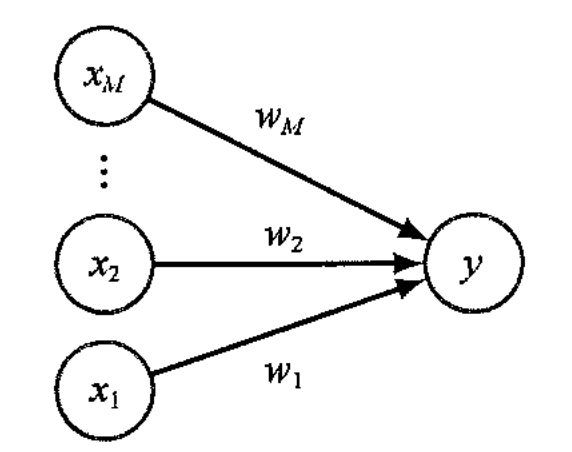
\includegraphics[width=0.33\textwidth]{ch01-fig1-14-simple-network.png}
  \caption{一个简单的神经网络模型，用于描述单个神经元的转换。多项式函数可以视为这个模型的一个特例}
  \label{figure:ch01-简单神经网络}
\end{figure}

\subsection{单层网络}\label{subsection:ch01-单层网络}

人工神经网络的历史大致可以根据其复杂程度划分为三个不同的阶段，这种复杂性是通过处理的“层数”来衡量的。由式\eqref{align:ch01-神经元预激活}和式\eqref{align:ch01-神经元激活}描述的简单神经网络模型可以视为具有单层处理能力，对应\cref{figure:ch01-简单神经网络}中的单层连接结构。在神经计算的历史长河中，感知机模型（Rosenblatt, 1962）无疑占据着举足轻重的地位，其激活函数 $f(\cdot)$ 是以下形式的阶跃函数：

\begin{definition}[感知机]\label{definition:ch01-感知机}
在\cref{definition:ch01-人工神经网络}中取激活函数为阶跃函数
\begin{align}
  f(a) =
  \begin{cases}
    0, & a \leqslant 0,\\
    1, & a > 0,
  \end{cases}
  \label{align:ch01-感知机激活}
\end{align}
所得的模型称为\textbf{感知机}（perceptron）（Rosenblatt, 1962）。
\end{definition}

% SUPPLEMENT: parent=definition:ch01-感知机; kind=motivation; location=紧随其后的 remark（重构新增）
\begin{remark}（重构新增）
阶跃函数把连续的预激活 $a$ 压成两个取值，因而感知机是一个“硬”判别器：它只回答输入落在超平面 $a=0$ 的哪一侧，而不给出置信程度。这既符合“神经元要么放电要么不放电”的简化图像，也使它的判别区域恰好是半空间，这一点是后面“单层网络能力局限”的根源。
代价是它几乎处处不可微：$f$ 在 $a\neq 0$ 处的导数恒为 $0$，在 $a=0$ 处不可导，因此无法用梯度信息来调整权重。Rosenblatt 的感知机学习算法靠的是“分错就按输入方向修正权重”这一离散规则，而不是梯度下降；这也解释了为什么\cref{subsection:ch01-反向传播}要把激活函数换成连续可微的函数。
\end{remark}

它可以视为一个简化的神经元放电模型，在该模型中，当且仅当总加权输入超过 $0$ 的阈值时，神经元才会放电。感知机由 Rosenblatt（1962 年）首创，他开发了一种特定的训练算法，该算法有一个有趣的特点，即如果存在一组权重值使得感知机能够完美分类其训练数据，则该算法保证在有限步数内收敛到这一解（Bishop, 2006）。除了学习算法之外，感知机还需要一个专用的模拟硬件，如\cref{figure:ch01-感知机硬件}所示。典型的感知机配置有多个处理层，但其中只有一层可以从数据中学习，因此感知机被认为是一个“单层”神经网络。

\begin{figure}[htbp]
  \centering
  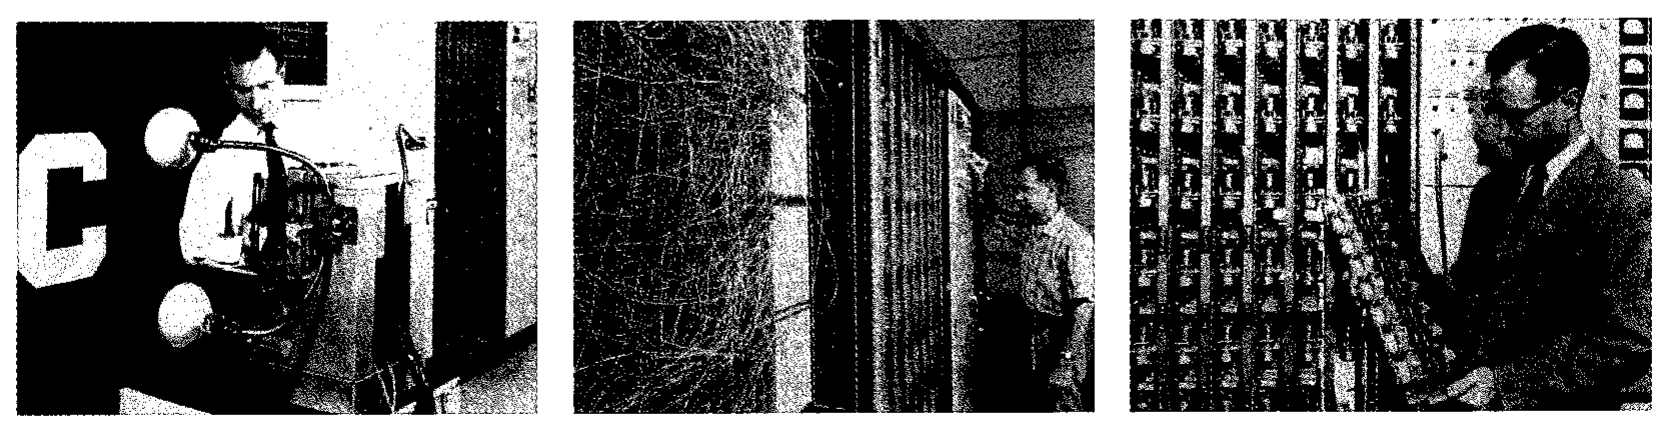
\includegraphics[width=0.95\textwidth]{ch01-fig1-15-mark1-perceptron.png}
  \caption{Mark 1 感知机硬件示意图。左图展示了使用简单的摄像系统获取输入，其中输入场景（在这种情况下是打印的字符）被强光照射，图像被聚焦在一个 $20\times 20$ 的硫化镉光电管阵列上，形成一幅原始的 $400$ 像素大小的图像。Mark 1 感知机还配备了一个接线板，如中间图所示，它允许尝试不同的输入特征配置。与现代数字计算机相比，这些通常是随机连接的，以展示感知机在没有精确连接的情况下进行学习的能力。右图展示了一个可学习权重机架，其中的每个权重都是使用旋转可变电阻器（也称电位器）实现的，由电动机驱动，从而允许通过学习算法自动调整权重值}
  \label{figure:ch01-感知机硬件}
\end{figure}

起初，大家惊叹于感知机能以类似大脑的方式从数据中学习。然而，这个模型也暴露出重大的局限性。Minsky and Papert（1969）分析了感知机的特性，并从数学上严格证明了单层网络的能力局限。他们还推测，这样的局限性将会扩展到具有多个可学习参数层的神经网络。尽管这一猜想后来被证明是极其错误的，但它在当时极大地打击了人们对神经网络模型的热情，并直接导致了 20 世纪 70 年代和 80 年代初学术界和工业界对神经网络领域缺乏足够的兴趣和资金投入。此外，由于缺乏有效的训练神经网络的算法，研究人员无法深入研究多层神经网络，因此像感知机这样的技术仅适用于单层模型。

\begin{remark}（重构新增）
“单层网络的能力局限”可以用一个具体反例说清。由式\eqref{align:ch01-神经元预激活}与式\eqref{align:ch01-感知机激活}，感知机的判据是 $a=\sum_i w_i x_i$ 是否超过阈值，若把阈值写成一个恒为 $1$ 的输入的权重，则判别边界是输入空间中的一张超平面，因此单层感知机只能实现\textbf{线性可分}的分类。
考察异或问题：输入 $(x_1,x_2)\in\{0,1\}^{2}$，要求 $y=1$ 当且仅当 $x_1\neq x_2$。设存在权重 $w_1,w_2$ 与阈值 $\theta$，使判别“$a>\theta$ 判为正类”完全正确。由 $(0,0)$ 属负类得 $0\leqslant\theta$；由 $(1,0)$ 与 $(0,1)$ 属正类得 $w_1>\theta\geqslant 0$、$w_2>\theta\geqslant 0$，从而 $w_1+w_2>2\theta\geqslant\theta$，即 $(1,1)$ 必被判为正类，与它属于负类矛盾。故单层感知机无法表示异或。
这一反例说明 Minsky 与 Papert 所指的局限是真的，但他们的外推——认为多层网络同样受限于此——是错的：只要在输入与输出之间加入带非线性激活的隐藏层，异或就可以被表示（两个隐藏单元已足够）。这正是“深度”带来的表达能力，也是\cref{subsection:ch01-深度网络}的历史起点。
\end{remark}

请注意，尽管感知机已经从实际机器学习应用中消失，但这个术语仍然流传下来，因此现代神经网络有时也称为多层感知机（Multi Layer Perceptron, MLP）。

\begin{definition}[多层感知机]\label{definition:ch01-多层感知机}
把\cref{definition:ch01-人工神经网络}中的多个单元按层组织、使前一层的输出作为后一层的输入的模型，整体称为\textbf{多层感知机}（Multi Layer Perceptron, MLP）——这是现代神经网络在历史上的另一名称。
\end{definition}

% SUPPLEMENT: parent=definition:ch01-多层感知机; kind=motivation; location=紧随其后的 remark（重构新增）
\begin{remark}（重构新增）
这个名字容易引起误解：现代的多层感知机既不是 Rosenblatt 的感知机（Rosenblatt 的感知机单元取式\eqref{align:ch01-感知机激活}的阶跃函数），也不限于单层；它指的是由多层可调权重的单元堆叠而成、通常用反向传播训练的网络。“感知机”一词在这里只剩下“每个单元先加权求和再作非线性变换”这一层含义。
之所以仍沿用旧名，是术语的历史惯性：\cref{subsection:ch01-单层网络}中单层模型失宠之后，多层版本沿用了同一名称以表明血统。阅读时只需记住：名字里的“感知机”不承诺任何能力上限，真正的限制来自层数、激活函数与训练算法。
\end{remark}

\subsection{反向传播}\label{subsection:ch01-反向传播}

对于训练具有多层可学习参数的神经网络问题，其解决方案来自微分学的应用以及基于梯度的优化方法。一项重要的改进是用具有非零梯度的连续可微激活函数取代了原有的阶跃函数（式\eqref{align:ch01-感知机激活}）。另一项关键的改进是引入了可微的误差函数，该函数能量化地评估在给定参数配置下模型对训练集中目标变量的预测效果。我们在\cref{section:ch01-一个教学示例}中利用平方和误差函数（式\eqref{align:ch01-平方和误差}）进行多项式拟合时，就已经接触到了此类误差函数的一个示例。

通过这些改进，我们现在得到了一个误差函数，它可以计算其关于网络模型中每一个参数的偏导数。现在我们可以着手考虑具有多层参数的网络结构了。\cref{figure:ch01-两层神经网络}展示了一个包含两层参数的简单网络模型。位于中间层的节点称为隐藏单元（hidden unit），因为它们的值不会出现在训练数据中，训练数据仅提供了模型的输入值和输出值。

\begin{definition}[隐藏单元]\label{definition:ch01-隐藏单元}
位于网络中间层、其取值既不出现在训练数据的输入中也不出现在训练数据的目标中的单元，称为\textbf{隐藏单元}（hidden unit）。
\end{definition}

% SUPPLEMENT: parent=definition:ch01-隐藏单元; kind=motivation; location=紧随其后的 remark（重构新增）
\begin{remark}（重构新增）
隐藏单元的存在是“深度”与“可学习特征”的连接点：训练数据只告诉网络输入是什么、输出应当是什么，中间层应当表示什么完全由训练过程自行决定。因此隐藏单元的值是模型内部的\textbf{隐变量}，而不是被观测的量。
这一条件也带来解释上的困难：正因为隐藏单元没有对应的监督信号，我们无法直接检查“它学到的表示是否正确”，只能通过最终误差间接判断。后文\cref{definition:ch01-表示学习}正是要从这个角度理解隐藏层的作用。
\end{remark}

\begin{figure}[htbp]
  \centering
  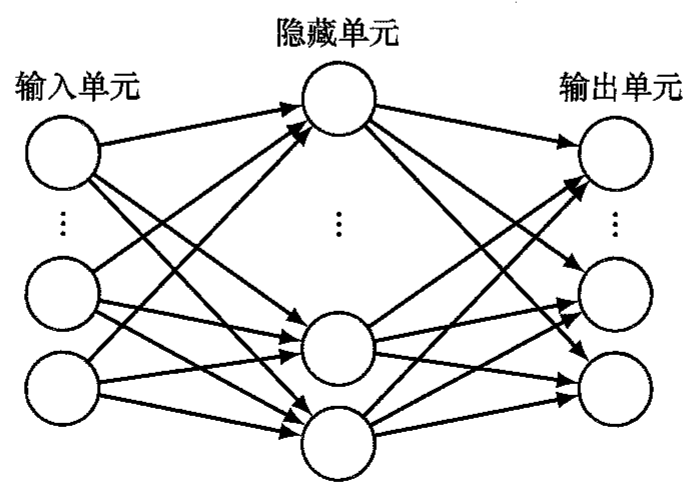
\includegraphics[width=0.55\textwidth]{ch01-fig1-16-two-layer-network.png}
  \caption{一个具有两层参数的神经网络（其中箭头表示神经网络中信息流的方向。每个隐藏单元和每个输出单元的计算形式分别由式\eqref{align:ch01-神经元预激活}和式\eqref{align:ch01-神经元激活}给出，其中激活函数 $f(\cdot)$ 是可微的）}
  \label{figure:ch01-两层神经网络}
\end{figure}

\cref{figure:ch01-两层神经网络}中的每一个隐藏单元和每一个输出单元均计算形如式\eqref{align:ch01-神经元预激活}和式\eqref{align:ch01-神经元激活}的函数值。对于一组给定的输入值，所有隐藏单元和输出单元的状态可以通过迭代地应用式\eqref{align:ch01-神经元预激活}和式\eqref{align:ch01-神经元激活}进行前向计算，在这个过程中，信息沿着箭头所指的方向在网络中逐层向前传递。由于这种信息流动的特点，此类模型也被称作前馈神经网络（feed-forward neural network）。

\begin{definition}[前馈神经网络]\label{definition:ch01-前馈神经网络}
若网络中每个单元只从其前一层的单元接收输入、并把输出送往其后一层的单元，信息沿单一方向逐层向前传递，则称这样的网络为\textbf{前馈神经网络}（feed-forward neural network）。
\end{definition}

% SUPPLEMENT: parent=definition:ch01-前馈神经网络; kind=motivation; location=紧随其后的 remark（重构新增）
\begin{remark}（重构新增）
“前馈”排除的是反馈连接：一旦某一层的输出被送回到更靠前的层，网络就具有了内部状态与时间动态，那属于循环网络，其计算与训练都要另行处理。前馈结构保证给定输入后各单元的值可以被依次算出，这正是前向计算能够“迭代地应用式\eqref{align:ch01-神经元预激活}与式\eqref{align:ch01-神经元激活}”的原因。
这一结构条件在后文的误差反向传播中还会再用一次：正因为信息流是单向的，误差才可以沿相反方向逐层回传而不产生循环依赖。若存在反馈连接，反向传播就需要展开时间或改用其他算法。
\end{remark}

为了训练这样的神经网络，我们首先使用随机数生成器初始化参数，然后使用基于梯度的优化技术进行迭代更新。这需要计算误差函数的偏导数，此操作可以通过误差反向传播（error backpropagation）过程中高效地完成（参见\cref{section:ch08-梯度计算}）。在反向传播中，信息从输出端向后通过神经网络流向输入端（Rumelhart, Hinton and Williams, 1986）。在机器学习领域，有许多不同的优化算法利用了待优化的函数的梯度，其中最简单和最常用的是随机梯度下降（stochastic gradient descent）法（参见\cref{section:ch07-梯度下降优化}）。

\begin{definition}[误差反向传播]\label{definition:ch01-误差反向传播}
计算误差函数关于网络各参数偏导数的一种高效方式称为\textbf{误差反向传播}（error backpropagation）：在该过程中，信息从输出端向后通过神经网络流向输入端，逐层给出误差函数对各层参数的偏导数（Rumelhart, Hinton and Williams, 1986）。
\end{definition}

% SUPPLEMENT: parent=definition:ch01-误差反向传播; kind=motivation; location=紧随其后的 remark（重构新增）
\begin{remark}（重构新增）
反向传播的实质是链式法则的系统化使用：先算出误差对输出的导数，再逐层用“上一层导数 × 本层局部导数”向前推进。它的效率来自复用——同一条回传路径上的中间量被所有更靠前的参数共享，因此一次反向遍历就能得到全部参数的梯度，计算量与一次前向计算同阶，而不是与参数个数同阶。
条件上，它要求每个单元的输出对其输入可微，这正是前面强调“用连续可微激活函数取代阶跃函数”的原因；若激活函数像式\eqref{align:ch01-感知机激活}那样几乎处处导数为零，回传的梯度会处处为零，参数就无法更新。此外反向传播只负责\textbf{算梯度}，如何用梯度更新参数是优化算法的事（参见\cref{section:ch07-梯度下降优化}）。
\end{remark}

能够训练具有多层权重的神经网络是一项重大突破，自 20 世纪 80 年代中期开始，这一突破再度引发了对该领域的研究热潮。这一时期，研究重心逐渐超越了单纯对神经生物学机制的模拟，而朝着构建更加严谨、更具原则性的理论基础的方向发展（Bishop, 1995b）。特别是，人们逐渐认识到，概率论和统计学中的核心思想在神经网络及机器学习领域扮演着至关重要的角色。一个关键的认识是，从数据中进行学习的过程不可避免地会引入一些背景假设，这些假设被称为先验知识（prior knowledge）或归纳偏置（inductive bias）。这些先验知识可以显式地融入模型设计之中，例如，可以设计一种特定的神经网络结构，使得皮肤病变的分类结果不依赖于图像中病变的具体位置；或者，它们也可以隐式地蕴含在模型的数学形式或其训练方法的选择中。

\begin{definition}[先验知识与归纳偏置]\label{definition:ch01-先验知识与归纳偏置}
从数据中进行学习的过程不可避免地会引入一些背景假设，这些假设称为\textbf{先验知识}（prior knowledge）或\textbf{归纳偏置}（inductive bias）。它们可以显式地融入模型设计（例如设计一种使分类结果不依赖病变位置的网络结构），也可以隐式地蕴含在模型的数学形式或其训练方法的选择中。
\end{definition}

% SUPPLEMENT: parent=definition:ch01-先验知识与归纳偏置; kind=motivation; location=紧随其后的 remark（重构新增）
\begin{remark}（重构新增）
为什么学习必然需要假设？因为有限个数据点可以被无穷多个函数同时拟合，若不对“哪些函数更可取”作出约定，就无法从无穷多个候选里挑出一个。先验知识正是这一约定的载体：它把假设空间从“所有函数”缩小到“我们愿意相信的函数”。
这也决定了偏置的两面性：偏置与数据规律相符时，学习效率大幅提高（例如卷积网络的平移等变性之于图像）；不相符时，再多的数据也难以纠正。因此“引入偏置”不是缺点而是必需，问题只在于偏置是否恰当——这一点在权重衰减的讨论中会以另一种形式出现（参见\cref{section:ch09-权重衰减}）。
\end{remark}

反向传播算法和基于梯度的优化技术显著提升了神经网络解决实际问题的能力。然而，研究人员注意到，在具有多层结构的神经网络中，通常只有最后两层的权重参数能够学习到有效的信息。除了少数例外，特别是用于图像分析的卷积神经网络模型（LeCun et al., 1998）（详见\cref{section:ch10-计算机视觉}），具有两层以上结构的网络模型鲜有成功的应用。这意味着此类网络模型不能有效解决太复杂的问题。为了在各种实际应用中获得令人满意的性能，人们通常要设计预处理步骤，将原始输入变量变换到一个新的特征空间中，希望在这个新的空间中机器学习任务能更容易解决。这种预处理步骤有时也被称为特征提取（feature extraction）。尽管这种人工特征提取的方法有时见效，但一个更理想的解决方案显然是直接从数据中自动学习出这些特征，而不是依赖于人工设计。

\begin{definition}[特征提取]\label{definition:ch01-特征提取}
把原始输入变量变换到一个新的特征空间、以使机器学习任务在该空间中更容易解决的预处理步骤，称为\textbf{特征提取}（feature extraction）。
\end{definition}

% SUPPLEMENT: parent=definition:ch01-特征提取; kind=motivation; location=紧随其后的 remark（重构新增）
\begin{remark}（重构新增）
特征提取的动机是“换一个坐标系看问题”：原始输入（如像素）与任务目标之间的关系往往极其复杂，而在经过恰当变换的空间里，同一任务可能近似线性可分。历史上这一步由人手工设计，其质量直接决定了后续分类器的上限。
它的局限也正是深度学习登场的原因：人工设计特征需要领域知识，且难以针对每个任务重新设计；更理想的做法是让模型自己学出这层变换，也就是把特征提取纳入可学习参数之中。条件上要注意，手工特征与学习到的表示并非互斥——前者可以作为后者的输入，或在数据极少时作为先验知识使用。
\end{remark}

到了 2000 年，当时的神经网络方法再次达到了它们能力的极限。研究人员开始探索替代神经网络的方法，如核方法、支持向量机、Gauss 过程等。尽管一些热情的研究人员继续追求真正有效训练多层神经网络的目标，但神经网络再次失宠。

\subsection{深度网络}\label{subsection:ch01-深度网络}

神经网络发展的第三个阶段，也是当前阶段，始于 21 世纪的第二个十年。一系列的突破使具有多层权重的神经网络得以有效训练，从而消除了这些技术先前的能力限制。具有多层权重的网络称为深度神经网络，专注于这类网络的机器学习子领域称为深度学习（deep learning）（LeCun, Bengio and Hinton, 2015）。

\begin{definition}[深度神经网络与深度学习]\label{definition:ch01-深度神经网络与深度学习}
具有多层权重的网络称为\textbf{深度神经网络}（deep neural network），专注于这类网络的机器学习子领域称为\textbf{深度学习}（deep learning）。
\end{definition}

% SUPPLEMENT: parent=definition:ch01-深度神经网络与深度学习; kind=motivation; location=紧随其后的 remark（重构新增）
\begin{remark}（重构新增）
“深”是相对的说法：\cref{definition:ch01-多层感知机}只要求有隐藏层，而“深度”强调的是隐藏层数量足够多、以致训练本身成为难点。因此深度学习的核心问题不是“如何定义深度”，而是“如何让很多层的权重同时被有效训练”——这正是\cref{subsection:ch01-反向传播}遗留、由本节后面的几项进展回答的问题。
条件上，深度并不自动带来好处：层数增加会使误差信号在反传中逐层衰减、使优化更难，也会放大过拟合风险。后文提到的残差连接、大规模数据与正则化，正是为了让“深”在实践上可行而引入的配套手段。
\end{remark}

深度学习发展历程中的一个关键性主题，是神经网络模型规模的显著扩张，这集中体现在模型参数数量的爆炸式增长上。20 世纪 80 年代，拥有数百或数千个参数的神经网络模型还较为普遍，但这一数字随后稳步攀升至数百万乃至数十亿规模。而目前最前沿的模型，其参数数量更是达到了惊人的一万亿（$10^{12}$）量级。拥有海量参数的神经网络模型需要相应规模的庞大数据集进行训练，才能确保在训练过程中为这些参数有效赋值。这种庞大模型与海量数据的结合，反过来也对模型训练过程的计算能力提出了更高的要求。

图形处理单元（Graphics Processing Unit, GPU）作为一种专为特定应用设计的处理器，最初是为了满足视频游戏等应用中对高速图形渲染的需求而开发的。随后人们发现 GPU 的架构能够很好地适配神经网络的训练需求。具体而言，神经网络中某一层的各个单元所执行的运算可以高度并行地进行，这与 GPU 所提供的大规模并行计算架构高度契合（Krizhevsky, Sutskever, and Hinton, 2012）。如今，规模最大的那些模型的训练任务，通常需要在包含数千块 GPU 的大规模计算集群上完成，这些 GPU 之间通过专用的高速网络进行通信。

\cref{figure:ch01-计算量增长}描绘了历年来训练最先进的神经网络模型所需计算量的演变趋势，图中显现出两个特征显著的增长阶段。纵轴采用指数标度，其单位为 petaflop/s-days。其中，一个 petaflop 代表每秒执行 $10^{15}$ 次（一千万亿次）浮点运算，而一个 petaflop/s 则表示每秒一千万亿次的浮点运算速率。因此，一个 petaflop/s-day 就代表以每秒一千万亿次的运算速率持续运行 $24$ 小时所对应的计算量，这大约等价于 $10^{20}$ 次浮点运算。由此可知，图中最上方的水平线对应着高达 $10^{24}$ 次的浮点运算量，真是让人惊叹。

\cref{figure:ch01-计算量增长}中的两个直线段显示了两个指数级的增长阶段。我们可以清楚地看到，从感知机时代直至 2012 年前后，计算需求的翻倍周期约为 2 年，这与摩尔定律所预测的计算性能增长的总体趋势基本吻合。然而，自 2012 年步入深度学习时代以来，计算需求再次呈现出指数级的增长态势，但这一次的翻倍周期锐减至仅 3.4 个月，这意味着计算能力每年增长高达 10 倍之多！

\begin{figure}[htbp]
  \centering
  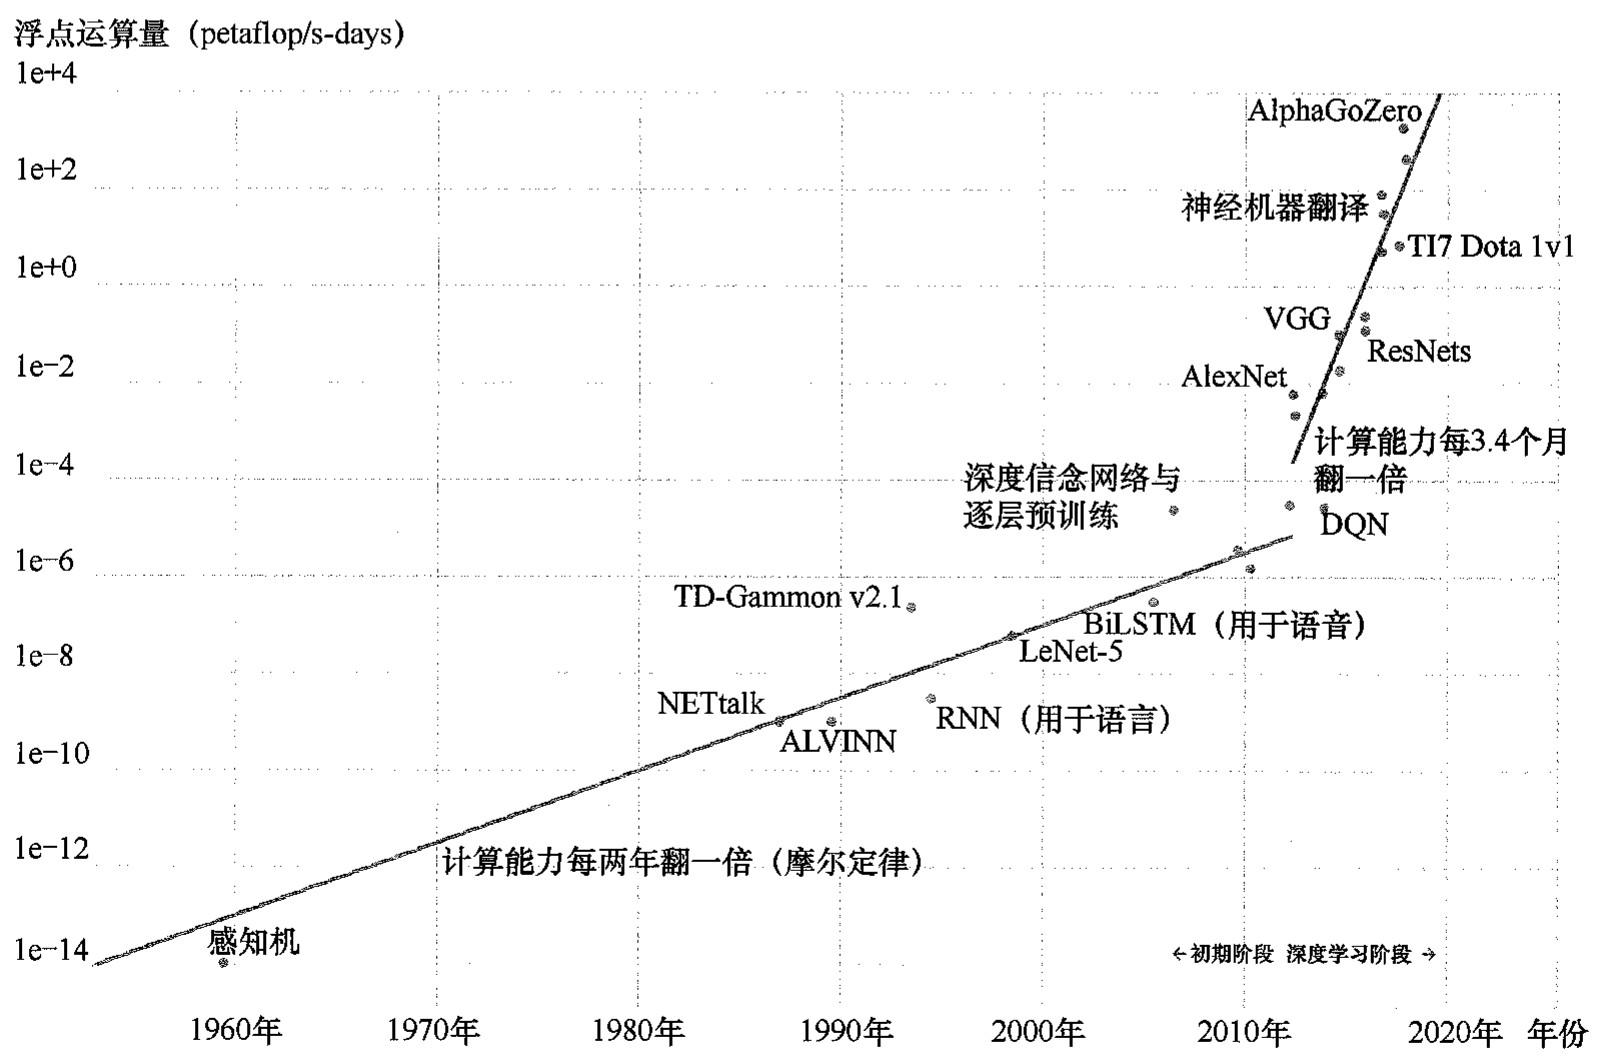
\includegraphics[width=0.95\textwidth]{ch01-fig1-17-compute-growth.png}
  \caption{训练最先进的神经网络所需的计算周期数（以 petaflop/s-days 为单位）与日期的关系，这里显示了两个不同的指数增长阶段（来自 OpenAI，经许可使用）}
  \label{figure:ch01-计算量增长}
\end{figure}

人们常常发现，通过架构创新或引入更复杂形式的归纳偏置而带来的性能改进，很快就会被简单地通过扩大训练数据量替代，同时伴随着相应的模型规模和用于训练的相关计算能力的扩展（Sutton, 2019）。大语言模型不仅在特定任务上表现更优，还可以用同一个训练好的神经网络解决更广泛范围的问题。大语言模型就是一个显著的例子，因为单个网络不仅拥有非凡的能力广度，甚至还能够胜过为解决特定问题而设计的专业网络（参见\cref{subsection:ch12-大语言模型}）。

我们已经了解到，网络的深度对于神经网络实现卓越性能至关重要。要理解深度神经网络中隐藏层的作用，一种有效的视角是表示学习（representation learning，也称表征学习）（Bengio, Courville, and Vincent, 2012）。在这种视角下，网络能够学习把原始输入数据转换成某种新的、富有语义信息的表示形式，从而显著降低后续网络层需要解决的问题的难度。这些学习到的内部表示还可以通过迁移学习技术被重新利用来解决其他相关问题，正如前文在皮肤病变分类任务中所展示的那样。一个有趣的发现是，用于处理图像的神经网络模型所学习到的内部表示，与在哺乳动物视觉皮层中观察到的神经表征惊人地相似（详见\cref{section:ch10-可视化训练好的CNN}）。

\begin{definition}[表示学习]\label{definition:ch01-表示学习}
把原始输入数据转换成某种新的、富有语义信息的表示形式，以降低后续网络层需要解决的问题的难度——这一视角与做法称为\textbf{表示学习}（representation learning，也称表征学习）。
\end{definition}

% SUPPLEMENT: parent=definition:ch01-表示学习; kind=motivation; location=紧随其后的 remark（重构新增）
\begin{remark}（重构新增）
表示学习把“特征工程”从人工搬到模型内部：隐藏层输出的就是输入的一种新表示，而它随参数一起被学习。判断一种表示是否有用，标准不是它像不像原始数据，而是它是否让后续任务变得更简单——在理想情形下，让原本高度非线性的判别问题在新空间中接近线性可分（\cref{definition:ch01-线性模型}）。
条件上，表示学习依赖“多层的复合”与“任务驱动的目标函数”：若没有足够深度，表示只能作一次简单变换；若没有明确的误差信号，所学表示就未必对目标任务有用。这也解释了为什么\cref{subsection:ch01-深度网络}所强调的规模化与表示学习是同一件事的两面：数据越多、模型越大，学到的表示才越通用。
\end{remark}

那些能够针对一系列下游任务进行适配或微调（fine-tuned）的大规模神经网络模型，称为基础模型（foundation model）。这些模型可以充分利用海量且多样化的数据集，从而构建出具有广泛适用性的通用模型（Bommasani et al., 2021）。

\begin{definition}[基础模型]\label{definition:ch01-基础模型}
能够针对一系列下游任务进行适配或微调（fine-tuned）的大规模神经网络模型，称为\textbf{基础模型}（foundation model）。
\end{definition}

% SUPPLEMENT: parent=definition:ch01-基础模型; kind=motivation; location=紧随其后的 remark（重构新增）
\begin{remark}（重构新增）
基础模型的要点是“一次训练、多处使用”：它先在海量且多样化的数据上得到一个通用模型，再通过适配或微调把它迁移到具体任务上（\cref{definition:ch01-预训练微调与迁移学习}）。因此它的价值不在某一项任务的精度，而在可被复用的广度。
条件上，“大规模”与“多样化”缺一不可：规模保证模型有足够容量吸收数据中的规律，多样化保证这些规律不局限于单一分布，从而使迁移到下游任务时仍然有效。这也带来代价——训练与推理的计算成本、以及下游任务与预训练分布不匹配时的性能下降，都需要另行处理。
\end{remark}

除了规模化这一因素外，还有其他若干进展也同样为深度学习的成功做出了重要贡献。例如，在传统的简单神经网络中，训练信号随着其在深度网络中逐层反向传播而逐渐衰减（详见\cref{section:ch09-残差连接}）。为了解决这一难题，一种名为残差连接（residual connection）的技术被引入网络架构中（He et al., 2015a），它极大地提高了对数百层深度的网络的训练效率。

\begin{definition}[残差连接]\label{definition:ch01-残差连接}
在深度网络中，为缓解训练信号逐层反传时的衰减而引入的一类跨层连接技术，称为\textbf{残差连接}（residual connection）（He et al., 2015a）。
\end{definition}

% SUPPLEMENT: parent=definition:ch01-残差连接; kind=motivation; location=紧随其后的 remark（重构新增）
\begin{remark}（重构新增）
残差连接的典型做法是让某一层的输出与该层的输入相加，使网络只需学习“在原有表示上需要改动多少”，而不必从头学出一个完整的变换。这样，即使中间各层的变换接近恒等，信息与梯度也能沿这条“直通”路径顺畅通过，深层网络的训练因此变得可行。
条件上，跨层相加要求两条通路的维数一致（否则需要先做线性投影），这也是实际架构中残差块通常保持通道数不变的原因。它并不增加模型的表达能力上限，改变的是\textbf{可优化性}——这一点与\cref{subsection:ch01-模型复杂度}中“模型容量”与“能否训练好”的区分是同一回事。
\end{remark}

另一项具有里程碑意义的进展是自动微分（automatic differentiation）方法的提出，该方法能够基于描述网络前向传播过程的代码，自动生成用于执行反向传播以计算误差函数梯度的代码。研究人员只需要显式地编写相对简洁的前向传播函数代码，就能够快速地探索和尝试不同的神经网络架构，并快速尝试不同的架构和多种组件的不同组合。

\begin{definition}[自动微分]\label{definition:ch01-自动微分}
能够基于描述网络前向传播过程的代码，自动生成用于执行反向传播以计算误差函数梯度的代码的方法，称为\textbf{自动微分}（automatic differentiation）。
\end{definition}

% SUPPLEMENT: parent=definition:ch01-自动微分; kind=motivation; location=紧随其后的 remark（重构新增）
\begin{remark}（重构新增）
自动微分既不是数值差分（用差商近似导数，精度与代价都受限），也不是符号求导（表达式会急剧膨胀），而是把\cref{definition:ch01-误差反向传播}的链式法则作用在程序本身上：前向计算被记录成一张计算图，反向遍历该图即得全部偏导数。
它的实际意义在于把“求梯度”从手工推导变成框架的职责，使研究者只需写好前向传播，就能尝试不同的架构与组件组合。条件上，它要求前向过程可被记录（即由可微的基本运算构成）；若代码中含有不可微或不可追踪的操作，自动微分同样会失效，这与\cref{definition:ch01-误差反向传播}对可微性的要求一致。
\end{remark}

此外，机器学习领域的很大一部分研究工作都是基于开源模式开展的，广大研究人员能够借助“他山之石”进行构建和拓展，从而进一步加快这个领域的创新步伐。

\end{document}
